\documentclass[tikz,border=14pt]{standalone}
\usepackage{lmodern}\usepackage{amsmath}\usepackage{amssymb}\usepackage{tikz}\usepackage{pgfplots}\pgfplotsset{compat=1.17}
\usetikzlibrary{calc,arrows.meta,positioning,patterns,decorations.markings,angles,quotes}
\definecolor{NebulaNavy}{HTML}{0B1F3A}
\definecolor{NebulaError}{HTML}{7952A3}
\definecolor{NebulaCheck}{HTML}{2E7D5B}
\definecolor{NebulaAmber}{HTML}{B47916}
\definecolor{NebulaGold}{HTML}{B77916}
\definecolor{NebulaLight}{HTML}{E4EAF0}
\definecolor{NebulaMuted}{HTML}{6E7E90}
\definecolor{NebulaNavyTwo}{HTML}{0B1F3A}
\definecolor{NebulaBG}{HTML}{F6F8FB}
\definecolor{NebulaSoft}{HTML}{E4EAF0}
\tikzset{
 nbline/.style={NebulaNavy,thick},
 nbdash/.style={NebulaNavy,thick,dashed},
 nbmass/.style={NebulaNavy},
 nbvec/.style={NebulaError,very thick,-{Stealth[length=2mm]}},
 nbvecb/.style={NebulaCheck,very thick,-{Stealth[length=2mm]}},
 nbaxis/.style={NebulaNavy,thick,-{Stealth[length=2mm]}},
}
\tikzset{nblabel/.style={NebulaNavy}}
\newcommand{\nbfuncplotlab}[9]{%
\pgfmathsetmacro{\nbyzero}{(0-(#3))/((#4)-(#3))}%
\begin{tikzpicture}
\begin{axis}[
  width=11.5cm, height=7.0cm,
  axis lines=middle,
  axis line style={NebulaNavy,-{Stealth[length=2mm]}},
  xmin=#1, xmax=#2, ymin=#3, ymax=#4,
  xlabel={#7}, ylabel={#8},
  xlabel style={at={(axis description cs:1.0,\nbyzero)},anchor=west,font=\small},
  ylabel style={at={(axis description cs:0.0,1.0)},anchor=south,font=\small},
  xtick distance=#5, ytick distance=#6,
  xticklabel style={font=\footnotesize,anchor=north,fill=white,inner sep=1.6pt},
  yticklabel style={font=\footnotesize,anchor=east,fill=white,inner sep=1.6pt},
  grid=both, grid style={NebulaMuted!45,very thin},
  tick style={NebulaNavy},
  clip=false
]
#9
\end{axis}
\end{tikzpicture}%
}
\usepgfplotslibrary{fillbetween}
\usetikzlibrary{backgrounds,3d,calc,intersections}
\begin{document}
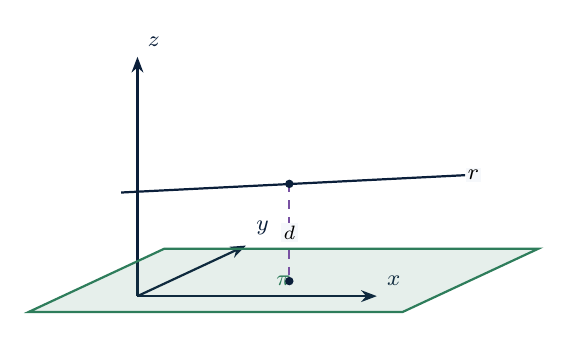
\begin{tikzpicture}[>={Stealth[length=2.2mm]},scale=0.95]
\draw[nbaxis] (0,0) -- (3.200,0.000) node[anchor=south west,font=\footnotesize]{$x$};
\draw[nbaxis] (0,0) -- (1.450,0.676) node[anchor=south west,font=\footnotesize]{$y$};
\draw[nbaxis] (0,0) -- (0.000,3.200) node[anchor=south west,font=\footnotesize]{$z$};
\draw[NebulaCheck,fill=NebulaCheck,fill opacity=0.12,thick] (-1.453,-0.211) -- (3.547,-0.211) -- (5.359,0.634) -- (0.359,0.634) -- cycle;
\node[NebulaCheck,font=\footnotesize] at (1.953,0.211) {$\pi$};
\draw[NebulaNavy,thick] (-0.219,1.385) -- (4.380,1.617);
\draw[NebulaError,dashed,thick] (2.030,1.501) -- (2.030,0.201);
\node[font=\scriptsize,fill=NebulaBG,inner sep=1pt] at (2.030,0.851) {$d$};
\node[font=\footnotesize,anchor=west,fill=NebulaBG,inner sep=0.8pt] at (4.380,1.617) {$r$};
\fill[NebulaNavy] (2.030,1.501) circle (1.6pt);
\fill[NebulaNavy] (2.030,0.201) circle (1.6pt);
\end{tikzpicture}
\end{document}
